\documentclass[12pt,a4paper]{article}
\usepackage{pgf}
\usepackage{svg}
\usepackage{tikz}
\usepackage{stanli}
\usepackage{afterpage}
\usepackage{multirow}
\usepackage{subfig}
\usepackage{pgfpages}
\usepackage{svg}
\usepackage{rotating}
\usepackage{pgfplots}

\pgfpagesdeclarelayout{boxed}
{
	\edef\pgfpageoptionborder{0pt}
}
{
	\pgfpagesphysicalpageoptions
	{%
		logical pages=1,%
	}
	\pgfpageslogicalpageoptions{1}
	{
		border code=\pgfsetlinewidth{2pt}\pgfstroke,%
		border shrink=\pgfpageoptionborder,%
		resized width=.9\pgfphysicalwidth,%
		resized height=.9\pgfphysicalheight,%
		center=\pgfpoint{.5\pgfphysicalwidth}{.5\pgfphysicalheight}%
	}%
}

\pgfpagesuselayout{boxed}

\usepackage[portuguese]{babel}

\usepackage[a4paper,top=2cm,bottom=1.5cm,left=1.5cm,right=1.5cm,marginparwidth=1.75cm]{geometry}

% Useful packages
\usepackage{amsmath}
\usepackage{graphicx}
\usepackage[colorlinks=true, allcolors=black]{hyperref}

\title{}
\author{}
\date{}

\begin{document}
	
	\newcommand{\subf}[2]{%
		{\small\begin{tabular}[t]{@{}c@{}}
				#1\\#2
		\end{tabular}}%
	}
	
	\begin{titlepage}
		\begin{center}
			\vspace*{3cm}
   
			\Huge
			\textbf{Projeto de Laboratórios de Informática III}
			\vspace{0.3cm}
			\Huge
   
			Fase 2
			\vspace{0.8cm}
   
			\large
			\vspace{1.5cm}
			\LARGE
			\vspace{1.5cm}
			\textbf{}
            \includegraphics[width=0.4\textwidth]{image.png}
			\vfill
			\vspace{1.0cm}
			\Large
			
		\end{center}
		\Large
		\begin{tabbing}
			\hspace*{1em}\= \hspace*{8em} \= \kill % set the tabbings
            \> Grupo: \textbf{44} \\
			\> Desenvolvido por: \textbf{Afonso Dionísio Santos, A104276} \\
            \>\>\textbf{Mário André Leite Rodrigues, A100109} \\
            \>\>\textbf{Pedro Figueiredo Pereira, A104082} \\
			
		\end{tabbing}
		
	\end{titlepage}
	
	\tableofcontents
	\newpage
    \section{Introdução}
    \hspace{0,6cm}Na unidade curricular de Laboratórios de Informática III, foi proposto realizar um projeto em C, para consolidar conhecimentos essenciais da linguagem prevista, assim como, desenvolvimento de aptidões no âmbito de engenharia de \textit{Software}, tais como modularidade e encapsulamento, estruturas dinâmicas de dados, validação funcional e medições de desempenho computacional. Prevê-se também a habilitação dos intervenientes relativamente à utilização de ferramentas essenciais ao desenvolvimento de projetos neste formato, nomeadamente, ferramentas de compilação, linkagem, depuração de erros, avaliação de desempenho, consumo de recursos e gestão de repositórios colaborativos. \\
        
    Após finalização com sucesso da primeira fase do projeto designado, que consistia em realizar \textit{parsing} e validação dos dados, criação de um modo \textit{Batch} e resolução de 6 \textit{queries}, iniciámos o desenvolvimento de uma solução que permitisse satisfazer todos os outros requisitos da aplicação, nomeadamente, capacitar a aplicação para realizar todas as dez \textit{queries}, testes funcionais
    e de desempenho, validação e filtragem do conjunto de dados fornecidos e criação de um modo \textit{Interativo}. \\

    Com a introdução da nova fase, surgiram novos desafios, deixou de estar isolada a única necessidade da realização das \textit{queries}, para se associar a um par essencial, a sua perfomance e desempenho em ambientes de maior exigência. A introdução de um \textit{dataset} com um tamanho 150 vezes superior ao inicialmente apresentado colocou todas as fragilidades ou soluções instáveis expostas, tornando mais relevantes as decisões tomadas e promovendo a nossa capacidade de resolução e auto-crítica. \\
        
    O relatório irá abordar decisões e estratégias pelas quais o grupo optou para concretização dos pontos referidos anteriormente com sucesso.
         
    \section{Desenvolvimento}
    \hspace{0,6cm}Dado todos os desafios referidos previamente, entre grupo, tomou-se a decisão de estabelecer algumas metas internas de gestão de recursos e qualidade do código implementado. Primeiramente, a restrição de utilização de memória que pretendemos estabelecer num valor inferior a 3500 megabytes, seguidamente, o comprometimento de executar as 500 \textit{queries} propostas pela equipa docente em menos de 150 segundos, ambos os valores baseados na plataforma de testes disponibilizada. Finalmente, a prontidão de manter e melhorar a qualidade do código e a sua documentação.

    \subsection{Arquitetura do projeto}

    \hspace{0,6cm}Esta sub-secção é dedicada à exposição das estruturas de dados utilizadas, diagrama de dependências dos módulos e dinâmica geral da aplicação, encapsulamento e documentação do código.
    
    \subsubsection{Estruturas de Dados}
    \hspace{0,6cm}

    Recapitulando a estrutura base utilizada na primeira fase, onde através de \textit{parsing} dos dados e posterior organização em estruturas, essencialmente dotadas de strings, procedíamos à consequente organização dos dados e resposta às \textit{queries}. Tal como descrito anteriormente, os novos requisitos incrementaram a dificuldade prevista, ainda assim, foi possível preservar as decisões iniciais, adaptando-as e melhorando a sua utilidade. \\

    Nesta segunda fase, foram criadas duas novas estruturas, o projeto está munido com cinco estruturas principais que são alimentadas à inserção dos dados, um \textit{GArray}, que armazena informações para apoio a estatísticas abstratas do \textit{user}, quatro \textit{Hashtables} que detêm os toda a informação útil presente nos ficheiros de entrada. \\

    Mantém-se a definição das estruturas, nas quais surgiram alterações às definições dos modelos que permitem a otimização a nível de memória, seguem as melhorias implementadas: \\

    Nos modelos atuais, implementámos 4 estratégias de redução de memória, mapeamento de strings (criação de duas \textit{Hashtables} com o objetivo de fazer corresponder um tipo char a uma string tendencialmente repetitiva no código), conversão de datas padrão e alguns ID's para inteiros (transformação do padrão YYYY/MM/DD para representação inteira YYYYMMDD), limitação nos ajustes dos tipo selecionados para representar a informação (Exemplos: \textit{hotel\_stars} é um valor inteiro de 1 a 5, logo usa-se o tipo char) e ordenação quantitativa do peso das representações nas estruturas (de acordo com a integridade da linguagem C, ordenámos as estruturas por, ou seja, char* menor que int menor que short int menor que char e booleano). \\

    Objetivamente, o primeiro ficheiro CSV a ser desconstruído para a memória foi o "/flights.csv", onde, optámos inicialmente por alocar apenas os dados úteis para resolução das queries. Como panorama final, apresentam-se os campos origin, destination, schedule\_departure\_date, schedule\_arrival\_date e real\_departure\_date como strings do tipo (char*), o campo flight\_id como inteiro do tipo (int), o campo total\_seats como inteiros reduzidos do tipo (short int) e finalmente, os campos airline e plane\_model como caractere do tipo (char).\\

    O segundo ficheiro a ser trabalhado foi o de "/passengers.csv", tal como na fase anterior optou-se por alocar os valores de flight\_id e user\_id como strings do tipo (char*).\\

    Segue-se a definição dos parâmetros do ficheiro de "/reservations.csv", onde, elaborámos as mesmas decisões e execuções do primeiro, finalmente, escolhemos o campo user\_id como string do tipo (char*), hotel\_id, begin\_date, end\_date e price\_per\_night como inteiros do tipo (int), os campos hotel\_name, hotel\_stars, city\_tax e rating são caracteres do tipo (char), finalmente o campo includes\_breakfast como booleano do tipo (bool).\\

    Por último, procedeu-se à desconstrução do ficheiro de "users.csv" através da aplicação da estratégia de uniformização de e manutenção dos estados iniciais e, como tal, definiram-se os campos user\_id, name, passport, country\_code e account\_creation como strings do tipo (char*), o campo birth\_date como inteiro do tipo (int) e os campos sex e account\_status como booleanos do tipo (bool).\\

    \subsubsection{Arquitetura Geral e Dependências}
    \hspace{0,6cm}
    
    Para cumprimento exímio das medidas de encapsulamento e modularidade, mantivemos a estrutura inicialmente acordada da aplicação, em que mais uma vez, embora não correspondendo inteiramente à definição habitual do modelo MVC (Model-View-Controller) adotámos alguns conceitos e nomenclatura. Pode observar-se na Figura 1 o diagrama de dependências que representa a nossa arquitetura e funcionamento do programa.

    \begin{center}
        \rotatebox{90}{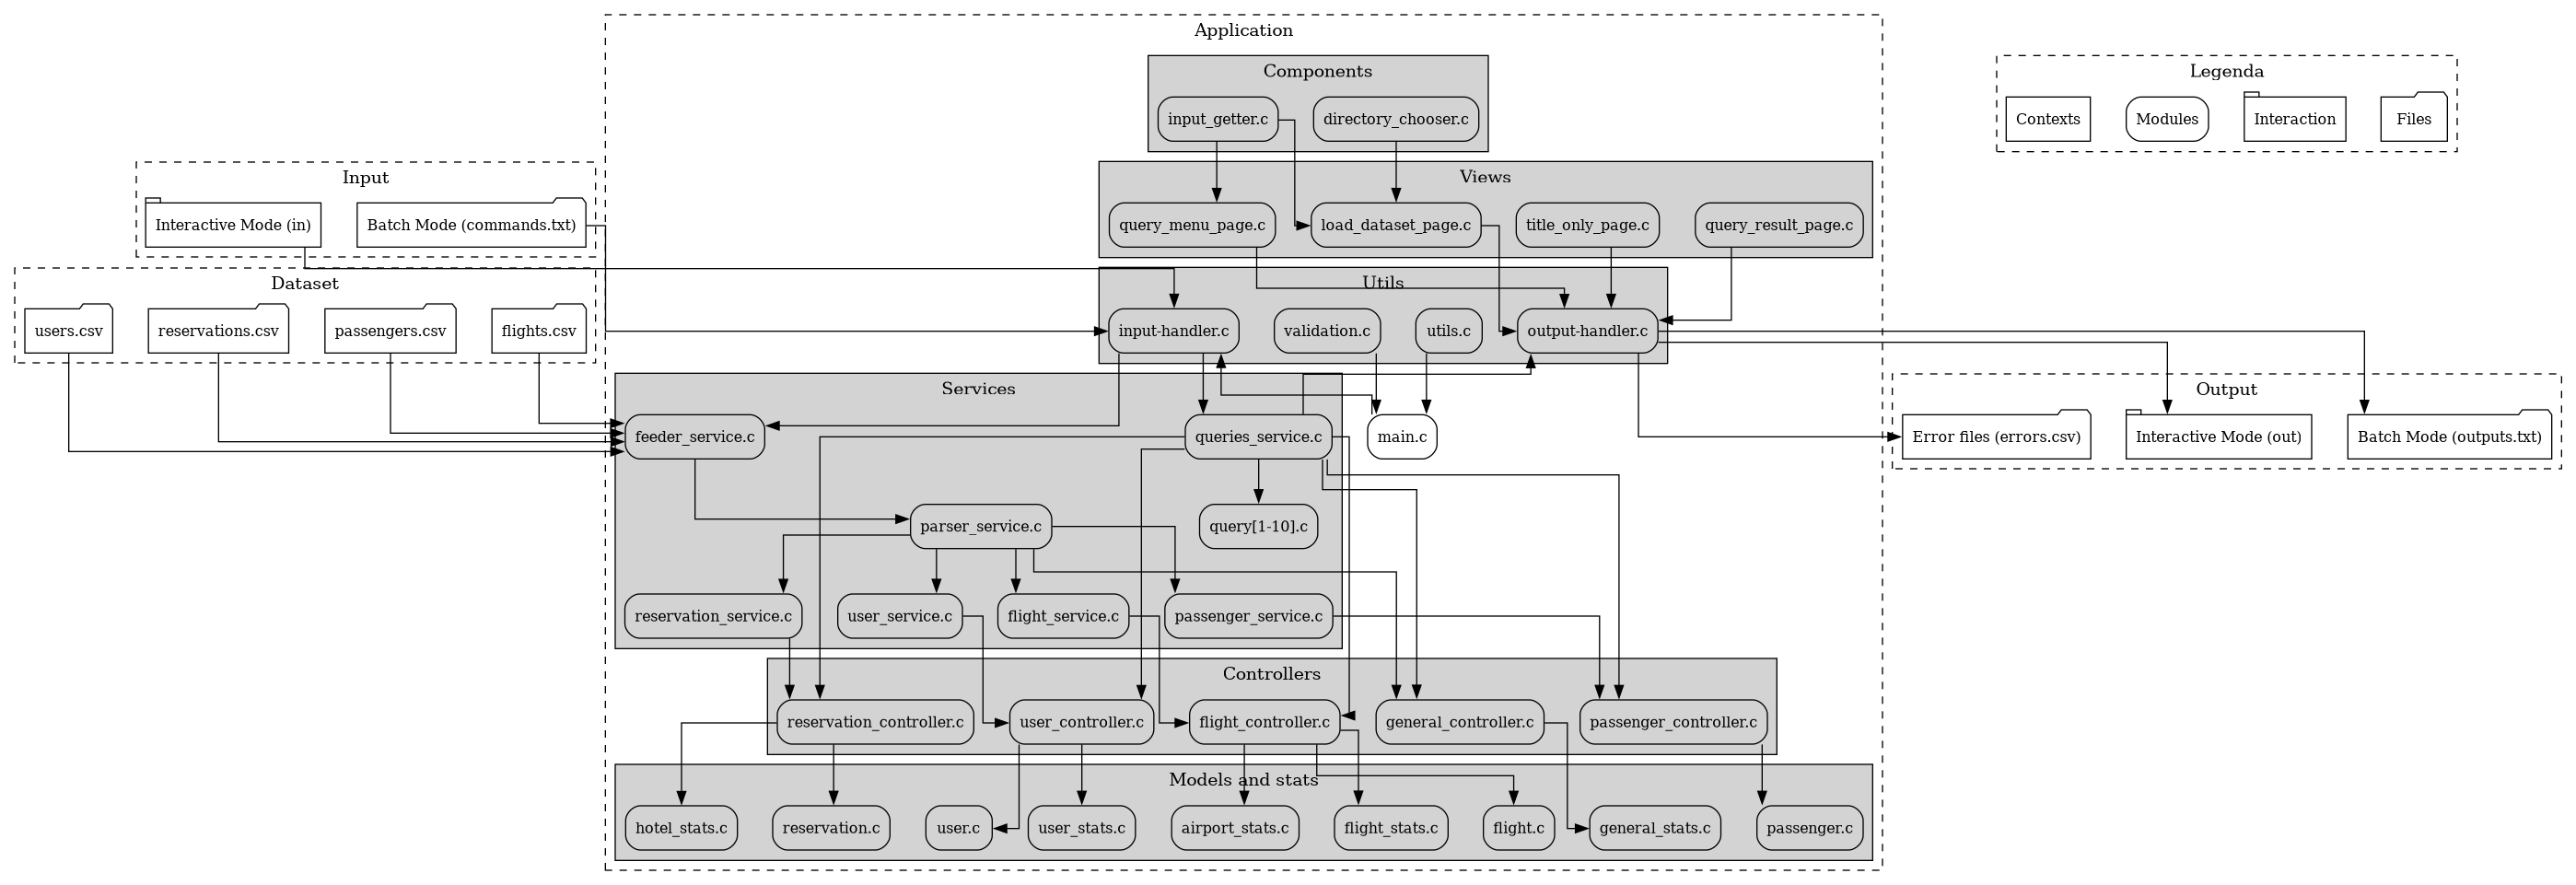
\includegraphics[scale=0.25]{diagrama.png}}
        \captionof{figure}{Diagrama de dependências e estrutura da aplicação.}
        \label{fig:diagrama}
    \end{center}


    \subsubsection{Encapsulamento}
    \hspace{0.6cm} De acordo com a importância do encapsulamento neste projeto, desde a primeira hora surgiu a necessidade de encapsular as estruturas, pertencentes aos diferentes módulos e contextos e as suas informações. \\
    
    De modo a assegurar este princípio e isolar todos os dados, recorremos a duplicação de memória a cada necessidade de utilização ou consulta de blocos de memória incorporativos das estruturas. Através de utilização dos padrões sugeridos de \textit{setters} e \textit{getters} para manipulação dos dados conseguimos garantir e respeitar o encapsulamento em todas as estruturas. \\

    Nesta segunda fase, mantivemos a prioridade de alinhamento com esta metodologia, continuando a manipulação de dados de acordo com a norma de forma a não ser possível o acesso ou alteração a dados externos ao próprio contexto e implementando as mesmas regras ao resto do código.
    
    \subsubsection{Documentação}
    \hspace{0.6cm} A documentação é um dos tópicos definidos como fundamentais desde da primeira vez que interagimos com o desafio proposto, associado a tal, foi também importante a garantia de boa prática de código, legibilidade e o explorar de recursos para facilitar a dinâmica do grupo. Toda a documentação está definida nos \textit{headers} através da norma \textit{Doxygen}, ferramenta a qual, permite a renderização para \textit{HTML} da informação de apoio. Foram também utilizados recursos como \textit{GitHub actions} e indentadores de código para complementar a documentação da aplicação.

    
    \subsection{Queries}
    \subsubsection{Query 1}
    \hspace{0,6cm}Na Query 1 foi mantida a decisão de implementação, sendo apenas ajustados alguns tipos inerentes a alterações de otimização geral.
    
    \subsubsection{Query 2}
    \hspace{0,6cm}Na Query 2, nesta segunda fase, foi imposta uma melhoria de legibilidade de código acompanhada da resolução de \textit{leaks} residuais presentes na primeira fase.

    \subsubsection{Query 3}
    \hspace{0,6cm}Na Query 3 foi mantida a decisão de implementação, sendo apenas ajustados alguns tipos inerentes a alterações de otimização geral.
       
    \subsubsection{Query 4}
    \hspace{0,6cm}Na Query 4, embora mantendo a estrutura atual melhorámos em ordenações desnecessárias de memória e incremento de desempenho das funções de comparação adjacentes.

    \subsubsection{Query 5}
    \hspace{0,6cm}A Query 5 tem como objetivo listar os voos com origem num aeroporto específico, entre duas datas fornecidas, ordenados pela data estimada de partida, do mais antigo para o mais recente. O código implementado utiliza estruturas de dados eficientes, como \textit{GArray} e \textit{structs}, para armazenar e organizar os resultados da consulta.\\

    No processo, são obtidas as estatísticas do aeroporto desejado, identificadas as respetivas partidas de voo e, em seguida, aplicados critérios de filtragem para selecionar apenas os voos que ocorrem dentro do intervalo de datas fornecido. Os resultados são então ordenados pela data estimada de partida, com um desempate baseado no identificador do voo em caso de datas iguais.\\

    O código também inclui funcionalidades para escrever os resultados no formato adequado para visualização ou exportação, permitindo uma integração eficaz com outros módulos do sistema. Esta abordagem garante a eficiência e correção na obtenção e apresentação dos resultados desejados para esta query específica.

    \subsubsection{Query 6}
    \hspace{0,6cm}Na Query 6, pretende-se que a sua principal funcionalidade seja listar os aeroportos com o maior número de passageiros em um determinado ano. O desafio reside na organização dos dados por ano e por aeroporto.\\

    Para resolver este problema, optámos por criar uma \textit{HashTable} organizada pelos anos. Dentro desta \textit{HashTable}, criamos outra estrutura organizada pelos aeroportos, contendo o número de passageiros correspondente a cada ano.\\

    Posteriormente, ao receber o ano como entrada, percorremos os aeroportos associados a esse ano. Utilizo uma estrutura auxiliar, \textit{GArray} para organizar os dados de forma decrescente, destacando os aeroportos com os maiores números de passageiros e finalizando a resolução da query.
    
    \subsubsection{Query 7}
    \hspace{0,6cm} Na Query 7, pretende-se que a sua principal funcionalidade seja listar um determinado número de aeroportos de forma decrescente de acordo com a mediana de atrasos desses aeroportos.\\
    
    Para resolver esse problema, adicionámos um novo parâmetro à estrutura dos aeroportos, que é um \textit{GArray}. Neste \textit{GArray}, serão armazenados os atrasos calculados durante a inserção dos dados.\\

     Posteriormente, itera-se sobre a \textit{HashTable} de forma a calcular a mediana de todos os aeroportos que são armazenados no \textit{GArray} auxiliar, este, contém o nome do aeroporto e a mediana dos atrasos correspondentes. Esses dados são, então, organizados por ordem decrescente.\\

     Este processo permite obter uma lista dos aeroportos com base na mediana de atrasos, proporcionando uma visão mais equilibrada em relação aos atrasos observados nos diferentes aeroportos.

    \subsubsection{Query 8}
    \hspace{0,6cm}A Query 8, ao contrário das outras queries, não escalou como planeado para o Dataset grande, pelo que, devido à falta de casos previstos, demonstrou deficiência na resolução da mesma. Para corrigir tal inconveniente, readaptou-se a estratégia para determinar as condições exatas necessárias ao bom funcionamento.

    \subsubsection{Query 9}
    \hspace{0.6cm}Na Query 9, embora mantendo a estrutura atual melhorámos em ordenações desnecessárias de memória e incremento de desempenho das funções de comparação adjacentes.

    \subsubsection{Query 10}
    \hspace{0.6cm}Na formulação da Query 10, o objetivo é calcular as estatísticas gerais do programa. A solução que desenvolvemos envolve a criação de uma \textit{HashTable} para armazenar as estatísticas gerais do programa.  \\

    Calculamos essas estatísticas durante a inserção de cada conjunto de dados. A chave para nossa \textit{HashTable} é um valor inteiro, onde para o ano corresponde a 20230000, para o mês corresponde a 20231200, e para o dia corresponde a 20231201, por exemplo. Para calcular os passageiros únicos, inserimos dados em uma \textit{HashTable} interna à \textit{HashTable} geral das estatísticas. Como a operação de busca (lookup) é executada em tempo constante, procuramos pelo usuário. Caso o retorno seja \textit{NULL}, inserimos o usuário e incrementamos uma unidade nos "unique passengers"; caso contrário, continuamos o funcionamento da aplicação sem realizar incrementos.

    \subsection{Validação de dados}
    \hspace{0,6cm}A validação de dados é uma etapa crucial no desenvolvimento do nosso projeto, garantindo a integridade e consistência das informações nos ficheiros de utilizadores, voos e reservas. Implementamos diversas verificações para assegurar que as datas seguem o formato adequado, respeitando os limites de meses e dias. Além disso, certificamo-nos de que as datas de término não são superiores às datas de início em utilizadores, voos e reservas, contribuindo para a coesão temporal dos dados.\\

    No que diz respeito aos emails dos utilizadores, estabelecemos um padrão rigoroso, exigindo a presença de um nome de utilizador e de um domínio com pelo menos um caractere. Verificamos também a consistência do código do país, garantindo que este é composto por duas letras. A validação de campos como o estado da conta dos utilizadores, o número de estrelas de um hotel, e o número de lugares disponíveis num voo, assegura que apenas valores aceitáveis são registados, evitando inconsistências e erros nos resultados das queries.\\

    Adicionalmente, desenvolvemos verificações específicas para campos como o número de estrelas de um hotel, a percentagem do imposto da cidade numa reserva e o preço por noite, assegurando que estes valores atendem aos critérios estabelecidos. Em casos de dados inválidos, procedemos à sua identificação e registo em ficheiros específicos, proporcionando transparência e facilitando a identificação de potenciais problemas. Este processo rigoroso de validação reflete o nosso compromisso com a qualidade e fiabilidade dos dados manipulados pela aplicação.
    
    \subsection{Modo Interativo}
    \hspace{0,6cm}O Modo Interativo do projeto oferece ao utilizador a flexibilidade de escolher entre duas opções para selecionar o conjunto de dados. Pode optar por inserir o caminho do ficheiro ou selecionar diretamente o próprio ficheiro. Após a seleção do conjunto de dados, o programa disponibiliza diversas opções de \textit{queries}, permitindo a inserção de input para obter respostas específicas.\\

    Para melhorar a experiência do utilizador, foi implementado um sistema de paginação em casos em que as respostas são extensas. Isso facilita a visualização e navegação pelos resultados, tornando a interação mais fluida.\\

    Além disso, a interface do Modo Interativo foi desenvolvida visando proporcionar uma experiência intuitiva. As opções de \textit{queries} são apresentadas de forma clara, e o utilizador é guiado de maneira eficiente para obter as informações desejadas.\\

    Este modo interativo não apenas recebe dados de ficheiros e os aloca na memória, mas também permite uma interação dinâmica, proporcionando uma experiência aprimorada aos utilizadores. A combinação de escolha de Dataset, opções de \textit{queries} e sistema de paginação contribuem para uma experiência rica e eficiente no uso do programa.

    \subsection{Testes de Funcionalidade}
    \hspace{0,6cm} Para assegurar a correta execução das nossas queries, implementámos uma abordagem de teste imediato. Após cada execução de query, realizamos uma comparação entre o output gerado e o output previsto para o respetivo input. \\

    Caso os resultados coincidam, a query é validada, e apresentamos ao utilizador o tempo decorrido durante a sua execução. No entanto, se houver discrepância entre o output gerado e o previsto, notificamos o utilizador, indicando o número da linha do erro e detalhando as diferenças encontradas. Este processo garante a robustez e fiabilidade do nosso sistema, permitindo uma depuração eficaz e uma melhoria contínua da aplicação.

    \subsection{Desempenho}
    \hspace{0,6cm}Nesta seção, apresentamos uma análise abrangente do desempenho obtido nas máquinas dos três membros do grupo durante o modo de testes. Essa avaliação é respaldada por dois gráficos e uma tabela que destacam os tempos médios de execução, além de fornecer detalhes sobre as especificações de cada máquina utilizada.\\

    Para garantir a confiabilidade dos resultados, foram realizadas 10 medições para cada conjunto de dados. Após essa fase, excluímos dois casos extremos para mitigar possíveis influências externas. Os valores apresentados na tabela são as médias diretas dos dados restantes, proporcionando uma visão precisa e representativa do desempenho das máquinas.\\

    A tabela inclui informações cruciais sobre o sistema operacional (O.S.), processador (CPU), número de cores/threads, capacidade de RAM e armazenamento em disco para cada máquina. Esses detalhes são essenciais para contextualizar os resultados e compreender o impacto das características de hardware nas execuções dos testes.\\

    Os gráficos subsequentes oferecem uma representação visual dos tempos de execução individuais para cada query em dois conjuntos de dados: pequeno e grande. Cada ponto nos gráficos representa o tempo de execução de uma query em uma máquina específica.\\

    Em suma, esta secção fornece uma análise abrangente do desempenho, abordando não apenas os resultados numéricos, mas também as especificações de hardware que influenciam diretamente no tempo de execução. Essa abordagem visa oferecer uma compreensão mais completa e informada do cenário de desempenho apresentado.

        \begin{figure}[p]
        \centering
        \begin{tabular}{|c|c|c|c|}
            \hline
            Máquina & 1 & 2 & 3 \\
            \hline
            O.S. & ArcoLinux & Arch & Arch \\
            \hline
            CPU & \parbox{3.8cm}{Intel i7-8750H (12) @4.100GHz (Hexa-core)} & 
                  \parbox{3.8cm}{Intel(R) Core(TM) i7-7820HQ CPU @2.90GHz (Quad-core)} & 
                  \parbox{3.8cm}{Intel(R) Core(TM) i7-1165G7 @2.80GHz (Quad-core)} \\
            \hline
            Cores/Threads & 12/24 & 8/16 & 8/16\\
            \hline
            RAM &  16GB & 8 GB & 8 GB \\
            \hline
            Disco & 1TB SSD M.2 & 256GB SSD M.2 & 512GB SSD M.2 \\
            \hline
            \multicolumn{4}{|c|}{Valores relativos ao dataset pequeno em segundos} \\
            \hline
            Query 1 & 0.000004 & 0.000006 & 0.000006 \\
            \hline
            Query 2 & 0.000025 & 0.000021 & 0.000019 \\
            \hline
            Query 3 & 0.000003 & 0.000004 & 0.000005 \\
            \hline
            Query 4 & 0.001156 & 0.001315 & 0.001374 \\
            \hline
            Query 5 & 0.000062 & 0.000059 & 0.000057 \\
            \hline
            Query 6 & 0.000009 & 0.000016 & 0.000013 \\
            \hline
            Query 7 & 0.000020 & 0.000029 & 0.000026 \\
            \hline
            Query 8 & 0.000017 & 0.000028 & 0.000025 \\
            \hline
            Query 9 & 0.000243 & 0.000646 & 0.000585 \\
            \hline
            Query 10 & 0.000007 & 0.000011 & 0.000009 \\
            \hline
            Tempo total & 0.320000 & 0.380000 & 0.340000 \\
            \hline
            \multicolumn{4}{|c|}{Valores relativos ao dataset grande em segundos} \\
            \hline
            Query 1 & 0.000030 & 0.000029 & 0.000027 \\
            \hline
            Query 2 & 0.000043 & 0.000138 & 0.000058 \\
            \hline
            Query 3 & 0.000004 & 0.000007 & 0.000004 \\
            \hline
            Query 4 & 0.169081 & 0.246641 & 0.170183 \\
            \hline
            Query 5 & 0.003741 & 0.005684 & 0.003998 \\
            \hline
            Query 6 & 0.000037 & 0.000039 & 0.000039 \\
            \hline
            Query 7 & 0.011839 & 0.012304 & 0.010992 \\
            \hline
            Query 8 & 0.002935 & 0.002273 & 0.003100 \\
            \hline
            Query 9 & 0.020832 & 0.023767 & 0.019976 \\
            \hline
            Query 10 & 0.000009 & 0.000012 & 0.000011 \\
            \hline
            Tempo total & 70.110000 & 89.630000 & 78.490090 \\
            \hline
        \end{tabular}
        \caption{Tempo de execução para máquinas do grupo}
        \label{tab:exemplo}
        \end{figure}
        
        \begin{center}
        \begin{tikzpicture}
          \pgfplotstableread[col sep=comma]{
            Query, Maquina1, Maquina2, Maquina3
            1, 0.000004, 0.000006, 0.000006
            2, 0.000025, 0.000021, 0.000019
            3, 0.000003, 0.000004, 0.000005
            4, 0.001156, 0.001315, 0.001374
            5, 0.000062, 0.000059, 0.000057
            6, 0.000009, 0.000016, 0.000013
            7, 0.000020, 0.000029, 0.000026
            8, 0.000017, 0.000028, 0.000025
            9, 0.000243, 0.000646, 0.000585
            10, 0.000007, 0.000011, 0.000009
          }\datatable
        
          \begin{axis}[
            title={Gráfico de desempenho individual (Dataset Pequeno)},
            xlabel={Número da Query},
            ylabel={Tempo de execução (s)},
            grid=major,
            legend pos=north est,
            xtick=data,
            xticklabels from table={\datatable}{Query},
            scale only axis,
          ]
        
          \addplot[mark=*, color=blue] table[x=Query, y=Maquina1] {\datatable};
          \addplot[mark=*, color=red] table[x=Query, y=Maquina2] {\datatable};
          \addplot[mark=*, color=green] table[x=Query, y=Maquina3] {\datatable};
        
          \legend{Máquina 1 (azul), Máquina 2 (vermelho), Máquina 3 (verde)}
        
          \end{axis}
        \end{tikzpicture}
        \end{center}

        \begin{center}
        \begin{tikzpicture}
          \pgfplotstableread[col sep=comma]{
            Query, Maquina1, Maquina2, Maquina3
            1, 0.000030, 0.000029, 0.000027
            2, 0.000043, 0.000138, 0.000058
            3, 0.000004, 0.000007, 0.000004
            4, 0.16081, 0.246641, 0.170183
            5, 0.003741, 0.005684, 0.003998
            6, 0.000037, 0.000039, 0.000039
            7, 0.011839, 0.012304, 0.010992
            8, 0.002935, 0.002273, 0.003100
            9, 0.020832, 0.023767, 0.019976
            10, 0.000009, 0.000012, 0.000011
          }\datatable
        
          \begin{axis}[
            title={Gráfico de desempenho individual (Dataset Grande)},
            xlabel={Número da Query},
            ylabel={Tempo de execução (s)},
            grid=major,
            legend pos=north est,
            xtick=data,
            xticklabels from table={\datatable}{Query},
            scale only axis,
          ]
        
          \addplot[mark=*, color=blue] table[x=Query, y=Maquina1] {\datatable};
          \addplot[mark=*, color=red] table[x=Query, y=Maquina2] {\datatable};
          \addplot[mark=*, color=green] table[x=Query, y=Maquina3] {\datatable};
        
          \legend{Máquina 1 (azul), Máquina 2 (vermelho), Máquina 3 (verde)}
        
          \end{axis}
        \end{tikzpicture}
        \end{center}

    \hspace{0,6cm}Com base nos resultados apresentados, é possível observar diferenças significativas no desempenho das máquinas do grupo durante a execução das queries nos conjuntos de dados pequeno e grande. No dataset pequeno, a Máquina 1 demonstrou tempos de execução notavelmente inferiores em comparação com as Máquinas 2 e 3. Essa discrepância pode ser atribuída à configuração mais robusta da Máquina 1, evidenciada pela presença de um processador Intel i7-8750H com 12 núcleos/24 threads, enquanto as Máquinas 2 e 3 possuem processadores quad-core. Além disso, a Máquina 1 possui uma capacidade de RAM superior (16GB), o que também pode contribuir para a melhoria do desempenho.\\

    No entanto, ao analisar o conjunto de dados grande, percebe-se que a Máquina 1 ainda mantém uma vantagem, mas as diferenças entre as máquinas tornam-se mais subtis. A Query 4, em particular, destaca-se com tempos de execução substancialmente mais longos, indicando uma possível área de otimização para todas as máquinas. A capacidade de armazenamento em disco também pode influenciar o desempenho em queries que envolvem acesso frequente ao armazenamento.\\

    Em suma, os resultados revelam a importância da configuração de hardware na eficiência do sistema, especialmente em operações intensivas de processamento de dados. A análise detalhada das especificações das máquinas fornece insights valiosos para compreender as variações no desempenho e identificar possíveis áreas de aprimoramento, contribuindo para a otimização futura da aplicação.
        
    \subsection{Dificuldades sentidas}      
    \hspace{0,6cm}O projeto enfrentou desafios na validação rigorosa de datas e na busca por algoritmos eficientes, especialmente em cenários de restrições rigorosas de tempo e memória. A implementação também exigiu a lógica para lidar com diferentes tipos de dados, como o processamento de valores decimais, e interfaces interativas intuitivas. A gestão de erros do usuário e a validação minuciosa dos arquivos de dados foram cruciais.\\

    A busca por soluções algorítmicas eficazes exigiu um equilíbrio entre complexidade computacional e eficiência operacional, sendo desafiador num contexto limitado temporalmente. A pressão temporal necessitou de uma abordagem estratégica para otimizar algoritmos sem comprometer a qualidade dos resultados.\\

    Assim, a implementação do projeto enfrentou desafios relacionados à validação de dados, processamento eficiente, garantia de uma experiência do usuário intuitiva e busca por algoritmos com bom desempenho em um ambiente restrito de tempo e memória. A solução envolveu uma abordagem cuidadosa para cada etapa, visando atender eficientemente às especificações do projeto.
        
    \section{Conclusão}
    \hspace{0,6cm}Em conclusão, o projeto representou um desafio multifacetado, abordando desde a validação rigorosa de dados até a busca por algoritmos eficientes em condições limitadas de tempo e memória. A implementação bem-sucedida exigiu uma cuidadosa harmonização entre a complexidade computacional e a eficiência operacional, destacando a importância da abordagem estratégica. A gestão de erros, interfaces intuitivas e a validação criteriosa dos dados contribuíram para uma solução robusta e alinhada com os objetivos do projeto. A jornada evidenciou a necessidade de adaptação e inovação para superar os desafios impostos, resultando numa implementação eficaz que atendeu às expectativas estabelecidas e cumprimento dos objetivos definidos na introdução.
        
\end{document} 
